\documentclass{article}
\usepackage[T1]{fontenc}
\usepackage{lmodern}
\usepackage{graphicx}
\usepackage{amsmath,amssymb}
\usepackage[a4paper,margin=2cm]{geometry}
\usepackage[absolute,overlay]{textpos}
\setlength{\TPHorizModule}{1mm}
\setlength{\TPVertModule}{1mm}
\usepackage[indonesian]{babel}
\usepackage{hyperref}
\setlength{\emergencystretch}{2em}
% unit: Halaman 71

\begin{document}

% === Halaman 71 (python/native) ===

Beberapa kesalahan umum karena tidak 

paham kriptografi

• Menganggap enkripsi = encoding, 

hashing, tokenisasi.

• Tidak paham perbedaan symmetric 

encryption dan asymmetric encryption, 

kapan menggunakan symmetric dan 

kapan menggunakan asymmetric 

encryption

71

Sumber gambar: Slide kuliah tamu dari Burman Noviansyah

% deskripsi: gambar native xref 479
\noindent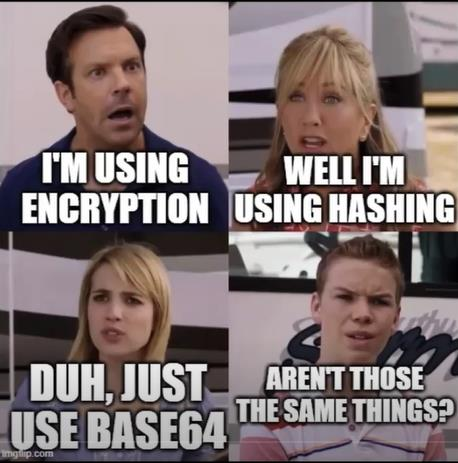
\includegraphics[width=0.85\textwidth]{../../images/python/page_071_img_01.jpeg}

\end{document}
